%
% A header that lets you compile a chapter by itself, or inside a larger document.
% Adapted from http://stackoverflow.com/questions/3655454/conditional-import-in-latex
%
%
%Use \inbpdocument and \outbpdocument in your individual files, in place of \begin{document} and \end{document}. In your main file, put in a \def \ismaindoc {} before including or importing anything.
%
% David Duvenaud
% June 2011
% 
% ======================================
%
%


\ifx\ismaindoc\undefined
	\newcommand{\inbpdocument}{
		\def \ismaindoc {}
		% Use this header if we are compiling by ourselves.
		\documentclass[a4paper,11pt,authoryear,index]{common/PhDThesisPSnPDF}
		
%\usepackage{draftwatermark}
%\SetWatermarkLightness{0.95}

% ******************************************************************************
% ****************************** Custom Margin *********************************

% Add `custommargin' in the document class options to use this section
% Set {innerside margin / outerside margin / topmargin / bottom margin}  and
% other page dimensions

\ifsetMargin
\else
    \RequirePackage[left=37mm,right=30mm,top=35mm,bottom=30mm]{geometry}
    \setFancyHdr % To apply fancy header after geometry package is loaded
\fi


%\chead{Unfinished draft}
%\cfoot{\texttt{Unfinished draft - compiled on \today{} at \currenttime}}

% *****************************************************************************
% ******************* Fonts (like different typewriter fonts etc.)*************

% Add `customfont' in the document class option to use this section

\ifsetFont
\else
    % Set your custom font here and use `customfont' in options. Leave empty to
    % load computer modern font (default LaTeX font).  

    \RequirePackage{libertine} 
\fi

% *****************************************************************************
% *************************** Bibliography  and References ********************

%\usepackage{cleveref} %Referencing without need to explicitly state fig /table

% Add `custombib' in the document class option to use this section
\ifsetBib % True, Bibliography option is chosen in class options
\else % If custom bibliography style chosen then load bibstyle here

   \RequirePackage[square, sort, numbers, authoryear]{natbib} % CustomBib

% If you would like to use biblatex for your reference management, as opposed to the default `natbibpackage` pass the option `custombib` in the document class. Comment out the previous line to make sure you don't load the natbib package. Uncomment the following lines and specify the location of references.bib file

% \RequirePackage[backend=biber, style=numeric-comp, citestyle=numeric, sorting=nty, natbib=true]{biblatex}
% \bibliography{References/references} %Location of references.bib only for biblatex

\fi


% changes the default name `Bibliography` -> `References'
\renewcommand{\bibname}{References}


% *****************************************************************************
% *************** Changing the Visual Style of Chapter Headings ***************
% Uncomment the section below. Requires titlesec package.

%\RequirePackage{titlesec}
%\newcommand{\PreContentTitleFormat}{\titleformat{\chapter}[display]{\scshape\Large}
%{\Large\filleft{\chaptertitlename} \Huge\thechapter}
%{1ex}{}
%[\vspace{1ex}\titlerule]}
%\newcommand{\ContentTitleFormat}{\titleformat{\chapter}[display]{\scshape\huge}
%{\Large\filleft{\chaptertitlename} \Huge\thechapter}{1ex}
%{\titlerule\vspace{1ex}\filright}
%[\vspace{1ex}\titlerule]}
%\newcommand{\PostContentTitleFormat}{\PreContentTitleFormat}
%\PreContentTitleFormat


% *****************************************************************************
% **************************** Custom Packages ********************************
% *****************************************************************************


% ************************* Algorithms and Pseudocode **************************

%\usepackage{algpseudocode} 


% ********************Captions and Hyperreferencing / URL **********************

% Captions: This makes captions of figures use a boldfaced small font. 
%\RequirePackage[small,bf]{caption}

\RequirePackage[labelsep=space,tableposition=top]{caption} 
%\renewcommand{\figurename}{Figure} %to support older versions of captions.sty
\captionsetup{belowskip=12pt,aboveskip=4pt}

% ************************ Formatting / Footnote *******************************

%\usepackage[perpage]{footmisc} %Range of footnote options 


% ****************************** Line Numbers **********************************

%\RequirePackage{lineno}
%\linenumbers

% ************************** Graphics and figures *****************************

%\usepackage{rotating}
%\usepackage{wrapfig}
%\usepackage{float}
\usepackage{subfig} %note: subfig must be included after the `caption` package. 


% ********************************* Table **************************************

%\usepackage{longtable}
%\usepackage{multicol}
%\usepackage{multirow}
%\usepackage{tabularx}


% ***************************** Math and SI Units ******************************

\usepackage{amsfonts}
\usepackage{amsmath}
\usepackage{amssymb}
%\usepackage{siunitx} % use this package module for SI units


% ******************************************************************************
% ************************* User Defined Commands ******************************
% ******************************************************************************

% *********** To change the name of Table of Contents / LOF and LOT ************

%\renewcommand{\contentsname}{My Table of Contents}
%\renewcommand{\listfigurename}{List of figures}
%\renewcommand{\listtablename}{List of tables}


% ********************** TOC depth and numbering depth *************************

\setcounter{secnumdepth}{2}
\setcounter{tocdepth}{2}

% ******************************* Nomenclature *********************************

% To change the name of the Nomenclature section, uncomment the following line

%\renewcommand{\nomname}{Symbols}


% ********************************* Appendix ***********************************

% The default value of both \appendixtocname and \appendixpagename is `Appendices'. These names can all be changed via: 

%\renewcommand{\appendixtocname}{List of appendices}
%\renewcommand{\appendixname}{Appndx}

		% All my custom preamble stuff.  Shouldn't overlap with anything in official-preamble


% Paths to figure and table directories.
\newcommand{\symmetryfigsdir}{figures/symmetries}
\newcommand{\topologyfiguresdir}{figures/topology}
\newcommand{\infinitefiguresdir}{figures/infinite}
\newcommand{\grammarfiguresdir}{figures/grammar}
\newcommand{\introfigsdir}{figures/intro}
\newcommand{\gplvmfiguresdir}{figures/gplvm}
\newcommand{\warpedfiguresdir}{figures/warped-mixtures}
\newcommand{\deeplimitsfiguresdir}{figures/deep-limits}
\newcommand{\quadraturefigsdir}{figures/quadrature}
\newcommand{\additivefigsdir}{figures/additive}
\newcommand{\decompfigsdir}{figures/decomp}
\newcommand{\examplefigsdir}{figures/worked-example}


\usepackage{bm}  % for warped mixtures - is this necessary?
\usepackage{booktabs}
\usepackage{tabularx}
\usepackage{multirow}
\usepackage{datetime}
\renewcommand{\tabularxcolumn}[1]{>{\arraybackslash}m{#1}}
\usepackage{relsize}
\usepackage{graphicx}
\usepackage{amsmath,amssymb,textcomp}
\usepackage{nicefrac}
\usepackage{amsthm}
\usepackage{tikz}
\usetikzlibrary{arrows}
\usetikzlibrary{calc}
\usepackage{nth}
\usepackage{rotating}
\usepackage{array}
\usepackage{fp}
\usepackage[hyperpageref]{backref}
\def\foo{\hspace{\fill}\mbox{}\linebreak[0]\hspace*{\fill}}
\renewcommand*{\backref}[1]{}
\renewcommand*{\backrefalt}[4]{%
\ifcase #1 %
%
\or
\foo(page #2)%
\else
\foo(pages #2)%
\fi
}

\usepackage{cleveref}
\crefname{equation}{equation}{equations}


%% For submission, make all render blank.
%%%%%%%%%%%%%%%%%%%%%%%%%%%%%%%%%%%%%%%%%%%%%%%%%%%%%%%%%%
%%%% EDITING HELPER FUNCTIONS  %%%%%%%%%%%%%%%%%%%%%%%%%%%
%%%%%%%%%%%%%%%%%%%%%%%%%%%%%%%%%%%%%%%%%%%%%%%%%%%%%%%%%%

%% NA: needs attention (rough writing whose correctness needs to be verified)
%% TBD: instructions for how to fix a gap ("Describe the propagation by ...")
%% PROBLEM: bug or missing crucial bit 

%% use \fXXX versions of these macros to put additional explanation into a footnote.  
%% The idea is that we don't want to interrupt the flow of the paper or make it 
%% impossible to read because there are a bunch of comments.

%% NA's (and TBDs, those less crucially) should be written so 
%% that they flow with the text.

\definecolor{WowColor}{rgb}{.75,0,.75}
\definecolor{SubtleColor}{rgb}{0,0,.50}

% inline
\newcommand{\NA}[1]{\textcolor{SubtleColor}{ {\tiny \bf ($\star$)} #1}}
\newcommand{\LATER}[1]{\textcolor{SubtleColor}{ {\tiny \bf ($\dagger$)} #1}}
\newcommand{\TBD}[1]{\textcolor{SubtleColor}{ {\tiny \bf (!)} #1}}
\newcommand{\PROBLEM}[1]{\textcolor{WowColor}{ {\bf (!!)} {\bf #1}}}

% as margin notes

\newcounter{margincounter}
\newcommand{\displaycounter}{{\arabic{margincounter}}}
\newcommand{\incdisplaycounter}{{\stepcounter{margincounter}\arabic{margincounter}}}

\newcommand{\fTBD}[1]{\textcolor{SubtleColor}{$\,^{(\incdisplaycounter)}$}\marginpar{\tiny\textcolor{SubtleColor}{ {\tiny $(\displaycounter)$} #1}}}

\newcommand{\fPROBLEM}[1]{\textcolor{WowColor}{$\,^{((\incdisplaycounter))}$}\marginpar{\tiny\textcolor{WowColor}{ {\bf $\mathbf{((\displaycounter))}$} {\bf #1}}}}

\newcommand{\fLATER}[1]{\textcolor{SubtleColor}{$\,^{(\incdisplaycounter\dagger)}$}\marginpar{\tiny\textcolor{SubtleColor}{ {\tiny $(\displaycounter\dagger)$} #1}}}

%\renewcommand{\LATER}[1]{}
%\renewcommand{\fLATER}[1]{}
%\renewcommand{\TBD}[1]{}
%\renewcommand{\fTBD}[1]{}
%\renewcommand{\PROBLEM}[1]{}
%\renewcommand{\fPROBLEM}[1]{}
%\renewcommand{\NA}[1]{}


% HUMBLE WORDS: shown slightly smaller when in normal text
% Thanks to Christian Steinruecken!

% HUMBLE WORDS: shown slightly smaller when in normal text
%
\makeatletter%
%\def\@humbleformat#1{{\fontsize{}{1em}\selectfont #1}}
%\def\@humbleformat#1{\textsmaller{#1}}%
\newlength{\nonHumbleHeight}
\def\@humbleformat#1{{\settoheight{\nonHumbleHeight}{#1}\resizebox{!}{0.94\nonHumbleHeight}{#1}}}%
\def\@idxhumbleformat#1{{\relscale{0.95}{#1}}}%
%\def\@humbleformat#1{{#1}}%
\def\declareHumble#1#2{%
  \expandafter\def\csname #1\endcsname{\@humbleformat{#2}}%
  \expandafter\def\csname s#1\endcsname{{#2}}%
  \expandafter\def\csname idx#1\endcsname{{\@idxhumbleformat{#2}}}%
}%
\def\humble#1{\@humbleformat{#1}}%
\def\idxhumble#1{\@idxhumbleformat{#1}}%
\makeatother%

% Convenient indexing for humble abbreviations
\def\humbleindex#1#2{\index{#1@\idxhumble{#1}}}



% TODO: Clean up duplicates
\declareHumble{ANOVA}{ANOVA}
\declareHumble{ARD}{ARD}
\declareHumble{BIC}{BIC}
\declareHumble{BMC}{BMC}
\declareHumble{bq}{BQ}
\declareHumble{CRP}{CRP}
\declareHumble{dirpro}{DP}
\declareHumble{HDMR}{HDMR}
\declareHumble{GAM}{GAM}
\declareHumble{GEM}{GEM}
\declareHumble{GMM}{GMM}
\declareHumble{gplvm}{GP-LVM}
\declareHumble{gpml}{GPML}
\declareHumble{GPML}{GPML}
\declareHumble{gprn}{GPRN}
\declareHumble{gpt}{GP}
\declareHumble{gp}{GP}
\declareHumble{HKL}{HKL}
\declareHumble{HMC}{HMC}
\declareHumble{ibp}{IBP}
\declareHumble{iGMM}{iGMM}
\declareHumble{iwmm}{iWMM}
\declareHumble{kCP}{CP}
\declareHumble{kCW}{CW}
\declareHumble{kC}{C}
\declareHumble{KDE}{KDE}
\declareHumble{kLin}{Lin}
\declareHumble{KPCA}{KPCA}
\declareHumble{kPer}{Per}
\declareHumble{kRQ}{RQ}
\declareHumble{kSE}{SE}
\declareHumble{kWN}{WN}
\declareHumble{Lin}{Lin}
\declareHumble{LBFGS}{L-BFGS}
\declareHumble{mcmc}{MCMC}
\declareHumble{MKL}{MKL}
\declareHumble{MLP}{MLP}
\declareHumble{MSE}{MSE}
\declareHumble{Per}{Per}
\declareHumble{RMSE}{RMSE}
\declareHumble{RQ}{RQ}
\declareHumble{SBQ}{SBQ}
\declareHumble{seard}{SE-ARD}
\declareHumble{sefull}{SE-\textnormal{full}}
\declareHumble{SEGP}{SE-GP}
\declareHumble{SE}{SE}
\declareHumble{SNR}{SNR}
\declareHumble{SSANOVA}{SS-ANOVA}
\declareHumble{SVM}{SVM}

\newcommand{\kSig}{\boldsymbol\sigma}

\def\subexpr{{\cal S}}
\def\baseker{{\cal B}}
\def\numWinners{k}

\def\ie{i.e.\ }
\def\eg{e.g.\ }
\def\etc{etc.\ }
\let\oldemptyset\emptyset
\let\emptyset 0




% Unify notation between neural-net land and GP-land.
\newcommand{\hphi}{h}
\newcommand{\hPhi}{\vh}
\newcommand{\walpha}{w}
\newcommand{\wboldalpha}{\bw}
\newcommand{\wcapalpha}{\vW}
\newcommand{\lengthscale}{w}

\newcommand{\layerindex}{\ell}



\newcommand{\gpdrawbox}[1]{
\setlength\fboxsep{0pt}
\hspace{-0.15in} 
\fbox{
\includegraphics[width=0.464\columnwidth]{\deeplimitsfiguresdir/deep_draws/deep_gp_sample_layer_#1}
}}



\newcommand{\procedurename}{ABCD}
\newcommand{\genText}[1]{{\sf #1}}



\newcommand{\asdf}{$^{\textnormal{th}}$}

\newcommand{\binarysum}{\sum_{\bf{x} \in \{0,1\}^D}}
\newcommand{\expect}{\mathbb{E}}
\newcommand{\expectargs}[2]{\mathbb{E}_{#1} \left[ {#2} \right]}
\newcommand{\var}{\mathbb{V}}
\newcommand{\varianceargs}[2]{\mathbb{V}_{#1} \left[ {#2} \right]}
\newcommand{\cov}{\operatorname{cov}}
\newcommand{\Cov}{\operatorname{Cov}}
\newcommand{\covargs}[2]{\cov \left[ {#1}, {#2} \right]}
\newcommand{\variance}{\mathbb{V}}
\newcommand{\vecop}[1]{\operatorname{vec} \left( {#1} \right)}

\newcommand{\covarianceargs}[2]{\Cov_{#1} \left[ {#2} \right]}
\newcommand{\colvec}[2]{\left[ \begin{array}{c} {#1} \\ {#2} \end{array} \right]}
\newcommand{\tbtmat}[4]{\left[ \begin{array}{cc} {#1} & {#2} \\ {#3} & {#4} \end{array} \right]}

%\newcommand{\covskinny}[2]{\var\!\left(#1\middle\vert#2\right)} 

\newcommand{\acro}[1]{{\humble{#1}}}
%\newcommand{\vect}[1]{\boldsymbol{#1}}
\newcommand{\vect}[1]{{\bf{#1}}}
\newcommand{\mat}[1]{\mathbf{#1}}
\newcommand{\pderiv}[2]{\frac{\partial #1}{\partial #2}}
\newcommand{\npderiv}[2]{\nicefrac{\partial #1}{\partial #2}}

\newcommand{\pha}{^{\phantom{:}}}

\newcommand{\argmin}{\operatornamewithlimits{argmin}}
\newcommand{\argmax}{\operatornamewithlimits{argmax}}

% The following designed for probabilities with long arguments

\newcommand{\Prob}[2]{P\!\left(\,#1\;\middle\vert\;#2\,\right)}
\newcommand{\ProbF}[3]{P\!\left(\,#1\!=\!#2\;\middle\vert\;#3\,\right)}
\newcommand{\p}[2]{p\!\left(#1\middle\vert#2\right)}
\newcommand{\po}[1]{p\!\left(#1\right)}
\newcommand{\pF}[3]{p\!\left(\,#1\!=\!#2\;\middle\vert\;#3\,\right)} 
\newcommand{\mean}[2]{{m}\!\left(#1\middle\vert#2\right)}



\newcommand{\valpha}{\boldsymbol{\alpha}}
\newcommand{\va}{\vect{a}}
\newcommand{\vA}{\vect{A}}
\newcommand{\vB}{\mat{B}}
\newcommand{\vb}{\vect{b}}
\newcommand{\vC}{\mat{C}}
\newcommand{\vc}{\vect{c}}
\newcommand{\vecf}{\boldsymbol{f}}
\newcommand{\vell}{\vect{\ell}}
\newcommand{\vepsilon}{\boldsymbol{\epsilon}}
\newcommand{\veps}{\boldsymbol{\epsilon}}
\newcommand{\ve}{\boldsymbol{\epsilon}}
\newcommand{\vf}{\vecf}
\newcommand{\vg}{\vect{g}}
\newcommand{\vh}{\vect{h}}
\newcommand{\vI}{\mat{I}}
\newcommand{\vK}{\mat{K}}
\newcommand{\vk}{\vect{k}}
\newcommand{\vL}{\mat{L}}
\newcommand{\vl}{\vect{l}}
\newcommand{\vmu}{\boldsymbol{\mu}}
\newcommand{\vone}{\vect{1}}
\newcommand{\vphi}{\boldsymbol{\phi}}
\newcommand{\vpi}{\boldsymbol{\pi}}
\newcommand{\vq}{\vect{q}}
\newcommand{\vR}{\mat{R}}
\newcommand{\vr}{\vect{r}}
\newcommand{\vsigma}{\boldsymbol{\sigma}}
\newcommand{\vSigma}{\mat{\Sigma}}
\newcommand{\vS}{\mat{S}}
\newcommand{\vs}{\vect{s}}
\newcommand{\vtheta}{\boldsymbol{\theta}}
\newcommand{\vu}{\vect{u}}
\newcommand{\vV}{\mat{V}}
\newcommand{\vW}{\mat{W}}
\newcommand{\vw}{\vect{w}}
\newcommand{\vX}{\mat{X}}
\newcommand{\vx}{\vect{x}}
\newcommand{\vY}{\mat{Y}}
\newcommand{\vy}{\vect{y}}
\newcommand{\vzero}{\vect{0}}
\newcommand{\vZ}{\mat{Z}}
\newcommand{\vz}{\vect{z}}


\newcommand{\netweights}{\alpha}
\newcommand{\vnetweights}{\valpha}

\newcommand{\He}{\mathcal{H}}
\newcommand{\normx}[2]{\left\|#1\right\|_{#2}}
\newcommand{\Hnorm}[1]{\normx{#1}{\He}}
\newcommand{\mmd}{{\rm MMD}}


\newcommand{\mf}{\bar{\vf}}

%\newcommand{\mf}{\mu} %{\bar{\ell}}
\newcommand{\lf}{f} % Likelihood function
\newcommand{\st}{_\star}

% from simpler log-bq writeup
\newcommand{\lftwo}{{\log \ell}}
\newcommand{\mftwo}{{\bar \ell}}
\newcommand{\loggp}{{\log\acro{GP}}}%| \bX, \vy )}}
\newcommand{\loggpdist}{{\acro{GP}(\lftwo)}}%| \vX, \vy )}}


\newcommand{\inv}{^{{\mathsmaller{-1}}}}
\newcommand{\tohalf}{^{{\mathsmaller{\nicefrac{1}{2}}}}}

\newcommand{\Normal}{\mathcal{N}}
\newcommand{\N}[3]{\mathcal{N}\!\left(#1 \middle| #2,#3\right)}
\newcommand{\Nt}[2]{\mathcal{N}\!\left(#1,#2\right)}
\newcommand{\NT}[2]{\mathcal{N}\!\left(#1,#2\right)}
\newcommand{\GPdist}[3]{\mathcal{GP}\!\left(#1 \, \middle| \, #2, #3 \right)}
\newcommand{\bN}[3]{\mathcal{N}\big(#1 \middle| #2,#3\big)}
\newcommand{\boldN}[3]{\text{\textbf{\mathcal{N}}}\big(#1;#2,#3\big)}
\newcommand{\ones}[1]{\mat{1}_{#1}}
\newcommand{\eye}[1]{\mat{E}_{#1}}
\newcommand{\tra}{^{\mathsf{T}}}
%\newcommand{\tra}{^{\top}}
%\mathsf{T}
\newcommand{\trace}{\operatorname{tr}}
\newcommand{\shift}{\operatorname{shift}}
\renewcommand{\mod}{\operatorname{mod}}
\newcommand{\deq}{:=}
\newcommand{\oneofk}{\operatorname{one-of-k}}
%\newcommand{\degree}{^\circ}

\newcommand{\GPt}[2]{\mathcal{GP}\!\left(#1,#2\right)}
%\newcommand{\GPt}[2]{\gp\!\left(#1,#2\right)}

\DeclareMathOperator{\tr}{tr}
\DeclareMathOperator{\chol}{chol}
\DeclareMathOperator{\diag}{diag}

\newenvironment{narrow}[2]{%
  \begin{list}{}{%
  \setlength{\topsep}{0pt}%
  \setlength{\leftmargin}{#1}%
  \setlength{\rightmargin}{#2}%
  \setlength{\listparindent}{\parindent}%
  \setlength{\itemindent}{\parindent}%
  \setlength{\parsep}{\parskip}}%
\item[]}{\end{list}}



\newcommand{\dist}{\ \sim\ }
\def\given{\,|\,}

% Table stuff
\newcolumntype{C}[1]{>{\centering\let\newline\\\arraybackslash\hspace{0pt}}m{#1}}
\newcolumntype{L}[1]{>{\raggedright\let\newline\\\arraybackslash\hspace{0pt}}m{#1}}
\newcolumntype{R}[1]{>{\raggedleft\let\newline\\\arraybackslash\hspace{0pt}}m{#1}}


\def\ie{i.e.\ }
\def\eg{e.g.\ }
\def\iid{i.i.d.\ }
%\def\simiid{\sim_{\mbox{\tiny iid}}}
\def\simiid{\overset{\mbox{\tiny iid}}{\sim}}
\def\simind{\overset{\mbox{\tiny \textnormal{ind}}}{\sim}}
\def\eqdist{\stackrel{\mbox{\tiny d}}{=}}
%\newcommand{\distas}[1]{\mathbin{\overset{#1}{\kern \z@ \sim}}}
%TODO: fix this - it worked outside the thesis!
\newcommand{\distas}[1]{\mathbin{\overset{#1}{\sim}}}

\def\Reals{\mathbb{R}}

\def\Uniform{\mbox{\rm Uniform}}
\def\Bernoulli{\mbox{\rm Bernoulli}}
\def\GP{\mathcal{GP}}
\def\GPLVM{\mathcal{GP-LVM}}




% Kernel stuff

\def\iva{\vect{\inputVar}}
\def\ivaone{\inputVar}
\def\inputVar{x}
\def\InputVar{X}
\def\InputSpace{\mathcal{X}}
\def\outputVar{y}
\def\OutputSpace{\mathcal{Y}}
\def\function{f}
\def\kernel{k}
\def\KernelMatrix{K}
\def\SumKernel{\sum}
\def\ProductKernel{\prod}
\def\expression{e}
\def\feat{\vh}

\newcommand{\kerntimes}{ \! \times \!}
\newcommand{\kernplus}{ \, + \,}


% Proof stuff
\theoremstyle{plain}
\newtheorem{theorem}{Theorem}[section]
\newtheorem{lemma}[theorem]{Lemma}
\newtheorem{prop}[theorem]{Proposition}
\newtheorem{proposition}{Proposition}
\newtheorem*{cor}{Corollary}

% For infinite bq
\newcommand{\iv}{\theta}
\newcommand{\viv}{\vtheta}

% For intro chapter
\newcommand{\funcval}{\vf(\vX)}
\newcommand{\testpoint}{{\vx^\star}}

\newcommand{\underwrite}[2]{{\underbrace{#1}_{\textnormal{#2}}}}



% For kernel figures
\newcommand{\fhbig}{2cm}%
\newcommand{\fwbig}{3cm}%
\newcommand{\kernpic}[1]{\includegraphics[height=\fhbig,width=\fwbig]{\grammarfiguresdir/structure_examples/#1}}%
\newcommand{\kernpicr}[1]{\rotatebox{90}{\includegraphics[height=\fwbig,width=\fhbig]{\grammarfiguresdir/structure_examples/#1}}}%
\newcommand{\addkernpic}[1]{{\includegraphics[height=\fhbig,width=\fwbig]{\grammarfiguresdir/additive_multi_d/#1}}}%
\newcommand{\largeplus}{\tabbox{{\Large+}}}%
\newcommand{\largeeq}{\tabbox{{\Large=}}}%
\newcommand{\largetimes}{\tabbox{{\Large$\times$}}}%
\newcommand{\fixedx}{$x$ (with $x' = 1$)}%


		% ************************ Thesis Information & Meta-data **********************

%% The title of the thesis
%\title{Structured Gaussian Process Models} 
%\title{Automatic Model Construction \\ through \\ Structured Gaussian Processes}
%\title{Automatic Model-Building \\ through \\ Structured Gaussian Processes}
%\title{Automatic Modeling \\ with \\ Structured Gaussian Processes}    
\title{Automatic Model Construction \\ with Gaussian Processes}
%\title{Automatic Model Construction}
%\title{Automating Statistical Model Construction}


%\texorpdfstring is used for PDF metadata. Usage:
%\texorpdfstring{LaTeX_Version}{PDF Version (non-latex)} eg.,
%\texorpdfstring{$sigma$}{sigma}

%% The full name of the author
\author{David Kristjanson Duvenaud}

%% Department (eg. Department of Engineering, Maths, Physics)
%\dept{Department of Engineering}

%% University and Crest
\university{University of Cambridge}
\crest{
\includegraphics[width=0.25\textwidth]{University_Crest}}

%% You can redefine the submission text:
% Default as per the University guidelines: This dissertation is submitted for
% the degree of Doctor of Philosophy
%\renewcommand{\submissiontext}{change the default text here if needed}

%% Full title of the Degree 
\degree{Doctor of Philosophy}
 
%% College affiliation (optional)
\college{Pembroke College}

%% Submission date
\degreedate{June 2014} 

%% Meta information
\subject{LaTeX} \keywords{{LaTeX} {PhD Thesis} {Engineering} {University of Cambridge}}



		\begin{document}
	}	
	\newcommand{\outbpdocument}[1]{

		% Fake chapters so references aren't broken
\label{ch:intro}                
\label{ch:kernels}
\label{ch:grammar}
\label{ch:description}
\label{ch:additive}
\label{ch:deeplimits}
\label{ch:discussion}
		%\bibliographystyle{common/CUEDthesis}
		\bibliographystyle{plainnat}
		\bibliography{references.bib}
		\end{document}
	}	
\else
	%If we're inside another document, no need to re-start the document.
	\ifx\inbpdocument\undefined
		\newcommand{\inbpdocument}{}
		\newcommand{\outbpdocument}[1]{}
	\fi
\fi

\inbpdocument

\newcommand{\infinitefiguresdir}{infinite-figures}


\chapter{Expressing Structure through Kernels}
\label{ch:kernels}

\section{Nonparametric Inference via Bayesian Quadrature}

We extend the approximate integration method of Bayesian Quadrature to infinite structured domains, introducing a new inference method for nonparametric models.% which is potentially exact in the limit.  
This method admits more flexible sampling schemes than Markov chains, for example active learning, and provides natural convergence diagnostics.  We give conditions necessary for consistency, and show how to construct kernels between structures which take advantage of symmetries in the likelihood function.  We demonstrate our inference method on both the Dirichlet process mixture model and the Indian buffet process.



\section{Introduction}

The central problem of probabilistic inference is to compute integrals over probability distributions of the form
\begin{equation}
	Z_{f,p} = \int f(\iv) p(\iv) d\iv
	\label{eqn:integral}
\end{equation}
Examples include computing marginal distributions, making predictions while marginalizing over parameters, or computing the Bayes risk in a decision problem.  Machine learning has produced a rich set of methods for computing these integrals, such as Expectation Propagation[cite], Variational Bayes[cite], and many variations of Markov chain Monte Carlo (\mcmc{} ) [cite Iain Murray].  

In non-parametric models, estimating \eqref{eqn:integral} is especially challending, as the domain of integration in is infinite-dimensional.  A variety of \mcmc{} methods have been developed to tackle this problem.  However, \mcmc{} has known weaknesses, such as difficulty diagnosing convergence, the requirement of a burn-in period, and difficulty obtaining samples from a given subset of possible $\theta$.

%Monte Carlo methods produce random samples from the distribution $p$ and then approximate integral \eqref{eqn:integral} by taking the empirical mean: $\hat{Z} = \frac{1}{N}\sum_{n=1}^{N}f(x_n)$ of the function evaluated at those points.  When exact sampling from $p$ is impossible or impractical, Markov chain Monte Carlo (MCMC) methods are often used. MCMC methods can be applied to almost any problem but convergence of the estimate depends on several factors and is hard to estimate \cite{CowlesCarlin96}. 
%
%For nonparametric models, which have potentially infinite latent structure, MCMC is the de facto standard method for inference.  [talk about EP and VB? For instance, \cite{miller2009variational} implements VB for IBP.  Maybe mention reversible jump MCMC  \cite{green1995reversible}]

%When performing inference in nonparametric models,

Bayesian quadrature (\bq{}) \cite{BZHermiteQuadrature}, also known as Bayesian Monte Carlo \cite{BZMonteCarlo}, is a model-based method of approximate integration.  \bq{} infers a posterior distribution over $f$ conditioned on a set of samples $f(\viv_s)$, and gives a posterior distribution on $Z_{f,p}$.  \bq{} remains a relatively unexplored integration method, and has so far only been used in low-dimensional, continuous spaces \cite{BZMonteCarlo}.

\paragraph{Summary of contributions} In this paper, we extend the \bq{} method to infinite, structured domains, introducing a new family of inference methods for non-parametric models.  We give conditions necessary for consistency.  We introduce kernels for inference problems using the Indian Buffet process and Dirichlet Proces mixture model which encode the many symmetries of the likelihood functions.

We then demonstrate the advantages of model-based inference on synthetic datasets, such as uncertainty estimates, flexibility in sampling methods, and post-hoc sensitivity analysis of prior and likelihood parameters.  We then discuss limitations of the framework as it stands.

\section{Bayesian Quadrature}

In contrast to \mcmc{}, a procedure which computes \eqref{eqn:integral} in the limit of infinite samples, Bayesian quadrature is a \emph{model-based} integration method.  This means that \bq{} puts a prior distribution on $f$, then conditions on some observations $f(\viv_s)$ at some query points $\viv_s$.  The posterior distribution over $f$ then implies a distribution over $Z_{f,p}$, which can be obtained by integrating over all possible $f$.  See Figure \ref{fig:bq_intro} for an illustration of Bayesian Quadrature.

\begin{figure}
\centering
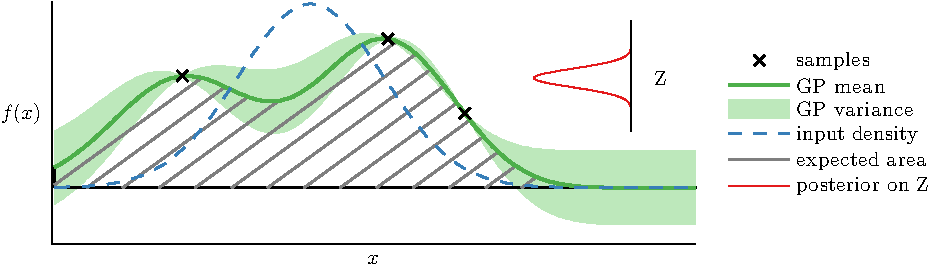
\includegraphics[width=0.8\linewidth]{\infinitefiguresdir/bq_intro5}
\caption{An illustration of Bayesian Quadrature.  The function $f(x)$ is sampled at a set of input locations.  This induces a Gaussian process posterior distribution on $f$, which is integrated in closed form against the target density, $p(\vx)$.  Since the amount of volume under $f$ is uncertain, this gives rise to a (Gaussian) posterior distribution over $Z_{f,p}$.}
\label{fig:bq_intro}
\end{figure}

It may seem circular to introduce an integral over an uncountable number of functions in order to solve what was originally an integral over a single function.  However, the \gp posterior has a simple form which makes integration possible in closed form in many cases.  If $f$ is assigned a Gaussian process prior with kernel function $k$ and mean $0$, then after conditioning on function evaluations $\vy = f(\iv_1) \dots f(\iv_N)$, we obtain:
%
\begin{align}
p(\vf(\iv\st)|\vy) = \N{\vf(\iv\st)}{\mf(\iv\st)}{\cov(\iv\st,\iv\st')}
\end{align}
where
\begin{align}
\label{eq:gp_mean} \mf(\vx\st) & = k(\iv\st, \iv_s) K^{-1} \vy \\
\label{eq:gp_var}\cov(\vx\st, \vx\st') & = k(\iv\st,\iv\st) - k(\iv\st, \viv_s) \vK^{-1} k(\viv_s, \iv\st)
\end{align} 
%
and $\vK_{mn} = k(\iv_m, \iv_n)$. 
%
Conveniently, the \gp{} posterior implies a closed form for the expectation and variance of \eqref{eqn:integral}:
%
%We now show how to compute the mean and variance of the Gaussian posterior distribution over $Z$, conditioned on the likelihood observations $\ell( \vtheta_s )$.  To do so, we need simply to integrate over possible likelihood functions $\ell(\theta)$.
%
\begin{align}
\expectargs{}{Z_{f,p} | \vy }&  = \expectargs{\gp(\lf | \vy )}{\int \lf(\theta)p(\theta)d\theta} %= \int\!\!\! \int\!\! \lf(\theta) p(\theta) d\theta p\left( \lf(\theta) \right) d \lf(\theta)\\
 %& = \int\! \mf(\theta) p(\theta) d\theta 
 = \left[ \int\!\! k(\theta, \vtheta_s) p(\theta) d\theta \right] \vK^{-1} \vy = \vz\tra \vK^{-1} \vy
\label{eq:gp_mean_symbolic} \\
\varianceargs{}{Z_{f,p}| \vy} & = \varianceargs{\textrm{prior}}{Z_{f,p}} - \vz\tra \vK^{-1} \vz
\label{eq:marg_var_symbolic}
\end{align}
%  \expectargs{\iv, \iv' \sim p}{k(\iv, \iv')}
%\end{align}
where 
\begin{align}
z_n & = \int\!\! k(\theta, \theta_n) p(\theta) d\theta \label{eq:little_z}\\
\varianceargs{\textrm{prior}}{Z_{f,p}} &  = \int\!\!\! \int\!\! k(\theta, \theta') p(\theta) p(\theta') d\theta d\theta' \label{eq:prior_var}.
\end{align}
For longer derivations, see the supplementary material.  This brings us to the one of the main technical constraints of this method:  Choosing a form for the kernel function $k(\theta, \theta')$ such that we can compute \eqref{eq:little_z} and \eqref{eq:prior_var} efficiently.  We must also set or integrate out any parameters of $k$.
%
 %Perhaps surprisingly, the posterior variance of $Z_{f,p}$ does not depend on the observed function values, only on the location of samples.  
%In practice, this method is slightly more complicated since we may wish integrate out parameters of $k$, which we do below.  % exactly for one parameter and numerically for others, by weighting against the likelihood of the \gp{}.


\subsection{BQ as an inference method}

%We might be interested in such quantities as the number of clusters, or the marginal density assigned by the model to some particular location $x$. 
If we assume that in \eqref{eqn:integral}, the form of $p(\theta)$ is such that we can compute $z_n$, then applying \bq{} is straighforward.  For example, in \cite{BZMonteCarlo}, \bq{} was used to solve problems where $p(\theta)$ was a Gaussian prior over parameters, and $f(\theta) = p( x | \theta )$ was a likelihood function, making $Z$ the \emph{model evidence}, a useful quantity when comparing models.

Typically, however, we are also interested in other quantities besides the model evidence, such as marginal distributions of latent parameter.  In that case, we must solve a more difficult integral, where $p(\theta) = p^* ( \theta | x )$ is a possibly unnormalized distribution of unknown form.
%
%If we sampled $\viv_s = \{\theta_1, \dots, \theta_N\}$ from the posterior $p(\theta | \vx)$ using MCMC, then we can estimate these quantities using a simple average:
%
%\begin{align}
%\expectargs{p(\theta | \vx)}{f(\theta)} & = \int f(\theta) p( \theta | x ) d\theta
%& \approx \frac{1}{N} \sum_{n=1}^{N} f( \theta_n )  \qquad \textrm{where}  \qquad \theta \sim p(\theta | \vx)
%\end{align}
%
%Instead [motivation needed], we will assign a \gp{} prior to the likelihood function $\ell(\theta) = p(\vx | \theta)$, then compute our expectations by computing
%
\begin{align}
\expectargs{p(\theta | \vx)}{f(\theta)} & = \int \!\! f(\theta) p(\theta | x ) d\theta 
% = \frac{ \int \! f(\theta) p( x | \theta ) p( \theta ) d\theta}{ \int\! p( x | \theta ) p( \theta ) d\theta} \\
& = \frac{1}{Z} \int \! f(\theta) p( x | \theta ) p( \theta ) d\theta \quad \textrm{where}  \quad  Z = \int \! p( x | \theta ) p( \theta ) d\theta
\label{eq:post_marginal}
\end{align}
%
%If we are only interested in relative expectations, then computing $Z$ is unnecessary.
%
%
%Next, we will show how to compute the unnormalized expectation using Bayesian quadrature: $\int \! f(\theta) p( x | \theta ) p( \theta ) d\theta$
%\begin{align}
%& = \int \!\!\! \int \!\! f(\theta) \ell(\theta) p( \ell( \theta ) ) d \ell( \theta ) d\theta
%\end{align}
%
%
%\section{Inference in Non-parametric Models}
%
%Inference in NP models requires integrating over infinite-dimensional spaces.  Typically, this is done by sampling a set of finite-sized latent structures from the approximate posterior via MCMC, and computing empirical expectations of the quantities of interest.
%
%When using \bq{}, the basic recipe will be to put a kernel between latent structures of arbitrary dimension.  This kernel will encode our model (of the likelihood functions)'s prior covariance between the likelihood function evaluated given each of the latent structures it is comparing.  Then, we analytically integrate the GP posterior over likelihood functions against the prior over different domains to obtain closed-form posterior distributions over those quantities.
%
%In the case that our sampled latent structures don't tell us much about the relative likelihood of different quantities, or we have too few samples, then our estimate will be bad.  However, unless the model is severely misspecified, the posterior variance of our estimator will be high, which will indicate that we are not yet certain about the value of our estimator.
%
%
% or the marginal likelihood of parameters of the prior, or even parameters of the likelihood.  Interestingly, in the latter two cases,  parameters of the likelihood\bq{} allows us to 
%
% If we wish to examine the effect of changing the parameters of the prior, we can simply recompute $\vz$ and examine the effect on the posterior over $Z$.  Similarily, if we wish to examine the effect of changing 
%
Integrals of this form can also be solved using Bayesian quadrature.  For a thorough treatment of this problem, see [Mike's BQR paper].  

This will show that \bq{} can be applied in several ways:  For instance, if we wish to perform inference about an unknown parameter $\tau$, we can include it as a variable to be integrated over by the \gp{}.  However, if for some technical reason this is difficult, we can also simply vary our extra parameter over some range, recomputing $\vy(\tau)$ and obtaining a marginal distribution over $Z_{f,p}$ for each value of $\tau$.  [Reference an experiment?]  This approach is useful for post-hoc sensitivity analysis.


\section{Guidelines for Constructing a Kernel}
\label{sec:kernels}

As pointed out above, one of the most important design decisions in \bq{} is the choice of kernel function $k(\theta, \theta')$, which specifies the prior covariance between the values of the likelihood function $p(\vx | \theta)$ and $p(\vx | \theta')$.  This function is somewhat analogous to the proposal distribution required to construct a Metropolis-Hastings sampler [cite].  In this section, we give guidance on how to construct an appropriate kernel.

The kernel typically should encode as much prior knowledge about the function being modeled as possible.  In regression problems, this usually amounts to specifying the smoothness properties of the function being modeled.  When doing inference, however, we typically know the likelihood function in closed form.  The more properties of the likelihood function we can encode in the kernel, the fewer samples we will need in order to  learn about the value of its integral.  In particular, we should encode any known symmetries:

\paragraph{Symmetry Encoding:} \label{des:pcor1} The prior correlation $\frac{k(\theta, \theta')}{\sqrt{k(\theta, \theta)} \sqrt{k(\theta', \theta')}}$ should equal 1 when $f(\theta) = f(\theta')$. That is to say, if two parameter settings are indistinguishable under the likelihood, our model can converge more quickly if it enforces that those likelihood values are identical.  This is another way of saying that the covariance function should encode all known symmetries. %  However, this is not a requirement for convergence in the limit. 
 % \item (Not sure about this one) More generally, the kernel function should respect any symmetries in the likelihood function.  That is, if $\ell(\theta') = \ell(\theta'')$, then $k(\theta, \theta') = k(\theta, \theta'')$.
%
%\end{enumerate}

The ability to encode symmetries in the kernel is one of the major advantages of \bq{} over Monte Carlo methods.  In unidentifiable models such as mixture models, often it is known that there exist many symmeteric modes in the posterior, which represents a major difficulty when computing model evidence.  By encoding these symmetries in the prior over likelihood functions, \bq{} neatly solves the problem of identifiability when estimating $Z_{f,p}$.


\subsection{Convergence}

In the existing \bq{} literature [cite only 4 papers], the integration problems considered have been low-dimensional, and the kernel function used has always been, to the best of the authors' knowledge, the squared-exponential kernel.  In that case, existing results on the consistency of \gp{} regression [cite consistency] imply that, under some conditions, the \bq{} estimator (a linear transform of the \gp{} posterior) is also consistent.  

For infinite-dimnensional spaces with complex kernels, it is more difficult to prove consistency, although the known structure of the likelihood functions may help.  In this section, we give conditions necessary for convergence.

First, the kernel must be positive-definite \cite{rasmussen38gaussian}.  In addition, in order to ensure convergence, we must have that the following condition holds:

%\subsection{Conditions}
%\begin{enumerate}
%
\paragraph{Identifiability:}  \label{cond:pcor_not1} The prior correlation $\frac{k(\theta, \theta')}{\sqrt{k(\theta, \theta)} \sqrt{k(\theta', \theta')}}$ must be less than 1 if it is possible that $f(\theta) \neq f(\theta')$. That is to say, if two values of the likelihood function can be different, our model must not enforce that those two function values are identical.
%  \item \label{cond:no_noise} (Not sure whether to keep this one)  If we add a diagonal noise term to our inference, it must go to zero as $N \rightarrow \infty$.  Otherwise, the posterior variance will not go to zero.
%\end{enumerate}
%
%
%
%
\begin{proposition}
The above condition is necessary to guarantee convergence of the BQ posterior to the true value of $Z$.
\end{proposition}
%
\begin{proof}[Proof sketch]
Consider a prior $p(\theta) = \frac{1}{2}\delta_{\theta_1}(\theta) + \frac{1}{2}\delta_{\theta_2}(\theta)$ where $\theta_1 \neq \theta_2$.  If the prior correlation between $f(\theta_1)$ and $f(\theta_2)$ is one, then after observing one of those two values, say $f(\theta_1)$ we have that $\expectargs{\gp}{Z} = f(\theta_1)$ and $\varianceargs{\gp}{Z} = 0$.  However if $f(\theta_1) \neq f(\theta_2)$, then $Z_0 = \frac{1}{2} f(\theta_1) + \frac{1}{2} f(\theta_2) \neq f(\theta_1)$.  Thus the estimator will have converged to the wrong hypothesis.
\end{proof}

%Note that if the prior correlation is one between two separate points, then after observing those to points, the Gram matrix becomes singular.  [However, maybe we can carefully cancel terms to avoid this?  Anyways, BMC with active learning will never choose points that would cause a singular matrix, because they would be perfectly uninformative].

For a more detailed proof, see the supplementary materical.  The statements in this section also hold for the problem of \gp{} regression in general, but are specially releveant for the problem of inferring likelihood functions over latent structures.  This is for two reasons:  First, likelihood functions over structures can typically by shown to have many symmetries.  Secondly, in the quadrature setting, we must learn about the function everywhere under the prior, not just in a small region or manifold, as is typical for regression problems.  Exploiting the symmetries of the likelihood function is both possible, and necessary for fast convergence.

%\subsection{Sufficiency}

%Although we give conditions necessary for convergence, and empirical results below indicate that \bq{} is consistent in these examples, we do not know of a proof of the consistency of \bq{} in infinite-dimensional spaces.  Gaussian process regression has been proved consistent in continuous finite spaces for popular kernels.[cite convergence paper].  Proving under which conditions the Bayesian Quadrature estimate is consistent would be a valuable further contribution, however such proofs typically depend on the details of both the functions being estimated, and the kernels being used to model them.



%Conditions \ref{cond:pcor_not1} and \ref{cond:no_noise} is sufficient to gaurantee the convergence of the BQ posterior to the true value of $Z$. 

\section{Inference in the Indian Buffet Process}

In this section, we construct a kernel and demonstrate the use of \bq{} for inference in an infinite latent model, the Indian buffet process.  The Indian buffet process (\ibp{}) \cite{griffiths2005infinite} is a distribution over binary matrices, usually used as a prior over latent features of a set of items.  The \ibp{} is nonparametric in the sense that the number of latent features is unbounded.
%
For example, in \cite{griffiths2005infinite}, a model of images is constructed where the entries of a binary matrix specify which objects appear in which images.  Although the number of objects is unknown beforehand, given a set of images, the flexible \ibp{} prior allows inference on both the number of objects, and their presence over the dataset.

Under an \ibp{} prior, the probability of seeing a matrix $\vZ$ with $K$ columns is
%
\begin{align}
P(\vZ|\alpha) & = \prod_{k=1}^K \frac{ \frac{ \alpha}{K} \Gamma(m_k + \frac{\alpha}{K}) \Gamma(N - m_k + 1)}{ \Gamma( N + 1 + \frac{\alpha}{K} ) }
\label{eq:IBP_prior}
\end{align}
%
where $m_k$ is the number of ones in column k, and $\alpha$ is the concentration parameter.  There is an unfortunate clash of notation here, where $Z_{f,p}$ denotes the model evidence, and $\vZ$ is used to denote a binary matrix.

To fully specify a model, we must also specify the likelihood of a set of observations $\vX$ given the latent structure, $p(\vX|\vZ)$.
For simplicity, we will use as a simple example the linear-Gaussian model from \cite{griffiths2005infinite}.  This model assumes the data is generated as $\vX = \vA \vZ + \ve$, with $A_{ij} \sim \NT{0}{\sigma_A}$ and $\ve_{ij} \sim \NT{0}{\sigma_X}$.  The features in $\vA$ are turned on and off for each row of $\vX$ by the entries of $\vZ$.   Conveniently, we can integrate out the matrix $\vA$ to obtain a collapsed likelihood:
\begin{align}
p(\vX | \vZ, \sigma_X, \sigma_A) = & \frac{\exp \left\{ - \frac{1}{2\sigma^2_X} \tr ( \vX^T ( \vI - \vZ ( \vZ^T \vZ + \frac{\sigma^2_X}{\sigma^2_A} \eye )^{-1} \vZ^T ) \vX ) \right\}}{(2\pi)^{\nicefrac{ND}{2}} \sigma_X^{(N-K)D} \sigma_A^{KD} | \vZ^T \vZ + \frac{\sigma_X^2}{\sigma_A^2} \vI |^\frac{D}{2}}
\label{eq:ibp_likelihood}
\end{align}
%
The goal of inference in the \ibp{} is usually do discover statistics about the matrices $\vZ$ and $\vA$, or to produce a predictive distribution over new rows of $\vX$.  In this paper, we will show how to [...]

\subsection{A kernel between binary matrices}

Here we give a kernel which satisfies the guidelines given in section \ref{sec:kernels}.  %An appropriate choice depends on the exact form of the likelihood function, as well as our expectations about the data.
%First, we will assign a kernel between individual feature vectors (columns of $\vZ$), denoted by $\vZ_{:,c}$:
%
%\begin{align}
%k(\vZ_{:,c_1}, \vZ'_{:,c_2}) = \sum_{n=1}^N \vZ_{n,c1} \vZ'_{n,c2}
%\end{align}
%
Since the likelihood in \eqref{eq:ibp_likelihood} does not depend on the order of columns of $\vZ$, we will construct a kernel function $k(\vZ, \vZ')$ which is also invariant to permutations over columns of both $\vZ$ and $\vZ'$:
%
\begin{align}
k(\vZ, \vZ') 
%& =  \sum_{k=1}^{K} \sum_{k'=1}^{K'} k(\vZ_{:,k}, \vZ'_{:,k'}) 
 =  \sum_{k=1}^{K} \sum_{k'=1}^{K'} \sum_{n=1}^N \vZ_{n,k} \vZ'_{n,k'} 
\label{eq:IBP_kernel1}
\end{align}
%
This kernel has the property that, for a given number of ones in $\vZ$ and $\vZ'$, it attains its maximum value when every element of some permutation of columns of $\vZ$ is equal to $\vZ'$ (i.e., they are in the same equivalence class).  [TODO: show that it achieves identifiability condition]

\subsection{Computing $z_n$ and the prior variance}

Now that we have defined our prior and kernel, we can compute the ``mini-normalization constants'', $z_1, \dots, z_n$, given by \eqref{eq:little_z}.  These quantities represent the expected covariance of the likelihood of a latent structure $\theta'$, with the likelihood of another structure drawn from the prior.

If matrices $\vZ$ and $\vZ'$ have $K$ and $K'$ columns respectively, then combining \eqref{eq:IBP_prior} and \eqref{eq:IBP_kernel1}, we have:
%
\begin{align}
z_n( \vZ ) & = \sum_{\vZ'} k(\vZ, \vZ') p(\vZ' | \alpha)
  = \sum_{\vZ'} \left[ \sum_{n=1}^N \sum_{k=1}^{K} \sum_{k'=1}^{K'} \vZ_{n,k} \vZ'_{n,k'} \right] \left[ \prod_{{k}^*=1}^K P({\vZ'}_{:,k^*} | \alpha ) \right] \\
% = \sigma^2_o \sum_{k'=1}^{K'} \sum_{n=1}^N \vZ'_{n,k'} \sum_{\vZ} \sum_{k=1}^{K} \vZ_{n,k} \prod_{k^*=1}^K P(\vZ_{:,k^*} | \alpha ) \\
% = \sum_{\vZ} \left[ \sum_{n=1}^N \sum_{k=1}^{K} \sum_{k'=1}^{K'} \vZ_{n,k} \vZ'_{n,k'} \right] \left[ \prod_{k^*=1}^K \int_0^1 \left( \prod_{i = 1}^{N} P(\vZ_{i,k^*} | \pi_{k^*} ) \right) p( \pi_{k^*} | \alpha ) d \pi_{k^*} \right]\\
%& = \sigma^2_o\sum_{k'=1}^{K'} \sum_{k=1}^{K} \sum_{n=1}^N \vZ'_{n,k'} \int_{\vzero}^{\vone} \sum_{\vZ} \vZ_{n,k} \prod_{k^*=1}^K \prod_{i = 1}^{N} P(\vZ_{i,k^*} | \pi_{k^*} ) p( \pi_{k^*} | \alpha ) d \pi_{k^*} \\
%& = \sum_{k'=1}^{K'} \sum_{k=1}^{K} \sum_{n=1}^N \vZ'_{n,k'} \int_0^1 \expectargs{ P(\vZ_{n,k} | \pi_{k} )}{ \vZ_{n,k} } p( \pi_{k} | \alpha ) d \pi_{k} 
% & = \sigma^2_o \sum_{k'=1}^{K'} \sum_{k=1}^{K} \sum_{n=1}^N \vZ'_{n,k'} \int_0^1 \pi_{k} p( \pi_{k} | \alpha ) d \pi_{k} \\
% & = \sigma^2_o \sum_{k'=1}^{K'} \sum_{k=1}^{K} \sum_{n=1}^N \vZ'_{n,k'} \frac{\frac{\alpha}{K}}{1 + \frac{\alpha}{K}} \\
& = \sum_{k=1}^{K} \sum_{n=1}^N \vZ_{n,k} \frac{\alpha}{1 + \frac{\alpha}{K'}} 
 = \alpha  \sum_{k=1}^{K} \sum_{n=1}^N \vZ_{n,k} \qquad \textrm{as $K' \rightarrow \infty$}
\label{eq:little_z_ibp}
\end{align}
%
See the supplementary material for longer derivations.
%
We can interpret \eqref{eq:little_z_ibp} as saying that the prior covariance of the likelihood $p(\vX|\vZ)$ with a randomly drawn likelihood $p(\vX|\vZ')$ is proportional to the number of ones in $\vZ$.  %Conveniently, this quantity does not depend on the number of columns of $\vZ$.
%As in \cite{griffiths2005infinite}, we take the infinite limit $K' \rightarrow \infty$.

%\subsection{Computing prior variance}

Next we compute the prior variance \eqref{eq:prior_var}, which follows a similar derivation.  This is the expected variance of $Z$ before we have seen any data.
\begin{align}
V_{\textrm{prior}} 
%= \int\!\!\! \int\! \! p(\theta) k(\theta, \theta') p(\theta') d\theta' d\theta
 = \sum_{\vZ'} \sum_{\vZ} p(\vZ | \alpha) k(\vZ, \vZ') p(\vZ' | \alpha) 
%  & = \sum_{\vZ'} \alpha \sigma^2_o \sum_{k'=1}^{K'} \sum_{n=1}^N \vZ'_{n,k'} p(\vZ' | \alpha) \\
%& = \alpha \sigma^2_o \sum_{k'=1}^{K'} \sum_{n=1}^N \sum_{\vZ'} \vZ'_{n,k'} \prod_{k^*=1}^K \int_0^1 \left( \prod_{i = 1}^{N} P(\vZ_{i,k^*} | \pi_{k^*} ) \right) p( \pi_{k^*} | \alpha ) d \pi_{k^*} \\
%& = \alpha \sigma^2_o \sum_{k'=1}^{K'} \sum_{n=1}^N \int_{\vzero}^{\vone} \sum_{\vZ'} \vZ'_{n,k'} \prod_{k^*=1}^K \prod_{i = 1}^{N} P(\vZ_{i,k^*} | \pi_{k^*} ) p( \pi_{k^*} | \alpha ) d \pi_{k^*} \\
%& = \alpha \sigma^2_o \sum_{k'=1}^{K'} \sum_{n=1}^N \int_0^1 \expectargs{ P(\vZ'_{n,k'} | \pi_{k'} )}{ \vZ'_{n,k'} } p( \pi_{k'} | \alpha ) d \pi_{k'} \\
%& = \alpha \sigma^2_o \sum_{k'=1}^{K'} \sum_{n=1}^N \int_0^1 \pi_{k'} p( \pi_{k'} | \alpha ) d \pi_{k'} \\
 = \frac{\alpha^2 N}{1 + \frac{\alpha}{K}} 
 = \alpha^2 N  \qquad \textrm{as $K \rightarrow \infty$}
\label{eq:prior_variance_ibp}
\end{align}
%
This form is intuitive:  it scales with the expected number of ones per row, $\alpha$.  As $\alpha$ or $N$ approach zero, the likelihood surface can be expected to become less varied, since there will be fewer ways that individual samples of $\vZ$ can differ.

%The posterior variance of $Z$ is simply $V_{\textrm{prior}} - \vz^T K^{-1} \vz$.



\section{Infinite Mixture Models}

In this section we develop a more general example, placing a kernel between mixture distributions.  This will allow us to perform model-based inference in Dirichlet process mixture models.

A finite mixture model with $k$ components gives a distribution over the observations $x$ as follows:
%
%\begin{align}
$p(x | \vpi, \vtheta) = \sum_{i = 1}^k \pi_i \p{x}{\theta_i}$
%\end{align}
%
where $\theta_i$ represents a single set of mixture parameters.  By specifying the form of $\theta$, we can perform inference in a wide variety of infinite mixture models, such as an latent Dirichlet allocation-type model, infinite mixture of regressors, or a mixture of Gaussians.

We will divide our derivation into two parts.  First, we will define a kernel between multinomial distributions, and derive \eqref{eq:little_z} and \eqref{eq:prior_var} for this kernel, leaving unspecified the kernel between individual mixture elements.  Then, we will continue the derivation for an infinite mixture of Gaussians.

\subsection{A Kernel Between Multinomial Distributions} 

Here we define a kernel between multinomial distributions, possibly of different dimension.  Here, $\vpi$ represents weights which sum to one, and $\theta$ the atoms of the multinomial distribution.
%
\begin{align}
k(\vpi, \vtheta, \vpi', \vtheta') = \sum_i^{n_\theta} \sum_j^{n_{\theta'}} \pi_i \pi_j' k_a( \theta_i, \theta_j')
\label{eq:multi_kernel}
\end{align}
%
where $k_a( \theta, \theta')$ specifies the covariance between individual atoms of the distribution.  Changing the order of mixture components, or splitting a given mixture component among two identical atoms, will not affect the value of this covariance function.  If $k_a( \theta_i, \theta_j')$ is a Mercer kernel, then so is \eqref{eq:multi_kernel}.

%\begin{itemize}
  %\item {\bf Finite Discrete Mixture Model}
%If we wish to provide a kernel between mixtures whose atoms are distinct, as in a discrete mixture model, we can set $k( \theta, \theta') = \delta( \theta, \theta' )$, and the kernel simply becomes a product of corresponding mixture weights.  However, this kernel will tend to zero as we increase the values $\theta$ with mass under the base measure.
  %
  %\item {\bf Infinite Mixture of Multinomials}
  %If we wish to provide a kernel between mixtures whose atoms are themselves multinomial distributions, then each $\theta$ is a mixture, and we can re-use the kernel inside of itself.  However, the atoms of the multinomials must be finite and shared, as in a bag-of-words model.
  %
  %\item {\bf Infinite Mixture of Gaussians} which we can also turn into a mixture of $t$, cauchy, etc simply by changing the likelihood function.
  %
%  \item {\bf Latent Dirichlet Allocation}
%  Here, the atoms are mixtures of multinomials???  Getting confused.
  %  
%\end{itemize}

%We stress that the kernel function is a modelling choice, and its form should depend on our expectations of the joint distribution over datasets that we expect to see.  Thus we needn't worry about finding the 'correct' form of kernel function for all datasets.



%\subsection{Computing $z_n$ and the prior variance}

If our mixture $\theta$ has $n_\theta$ components, then
%
\begin{align}
\nonumber  
z(\vpi, \vtheta) & = \int\!\!\! \int\!\! k(\vpi, \vtheta, \vpi', \vtheta') p(\vtheta') p(\vpi') d\vtheta' d\vpi' = \int\!\!\! \int\!\! \left[ \sum_{i=1}^{n_\theta} \sum_{j=1}^{n_{\theta'}} \pi_i \pi_j' k(\theta_i, \theta_j') \right] \left[ \prod_a^{n_{\theta'}} p(\theta'_a ) \right] p(\vpi') d\vtheta' d\vpi' \\
%& = \int \sum_{i=1}^{n_\theta} \sum_{j=1}^{n_{\theta'}} \pi_i \pi_j' \int\! k(\theta_i, \theta_j') \left[ \prod_a^{n_\theta} p(\theta_a) d\theta_a \right] p(\pi) d\pi\\
& = \int \sum_{i=1}^{n_\theta} \sum_{j=1}^{n_{\theta'}} \pi_i \pi_j' \underbrace{\int\! k(\theta_i, \theta_j') p(\theta'_j) d\theta'_j}_{z_a(\theta_i)} p(\vpi') d\vpi'
%& = \int \sum_{i=1}^{n_\theta} \sum_{j=1}^{n_{\theta'}} \pi_i \pi_j' z_k(\theta_j') p(\pi) d\pi \\
% & =  \int \sum_{j=1}^{n_{\theta'}} \pi_j' z_k(\theta_j') \underbrace{\sum_{i=1}^{n_\theta} \pi_i }_{\textrm{sums to one}} p(\pi) d\pi \\
 =  \sum_{i=1}^{n_{\theta}} \pi_i z_a(\theta_i)
\label{eq:little_z_dp} \\
%\end{align}
%
%Next, we compute the prior variance:
%
%\begin{align}
\varianceargs{\textrm{prior}}{Z_{f,p}} & = 
\int\!\!\! \int\! \! z( \pi, \theta) p(\theta) p(\pi) d\theta d\pi
%\int\!\!\! \int\! \! p(\theta) p(\pi) k(\pi, \theta, \pi', \theta') p(\theta') p(\pi')d\theta' d\pi d\theta d\pi'
% & = \int \sum_{j=1}^{n_{\theta'}} z(\theta_j') p(\theta') d\theta' \\
% = \int\!\!\! \int \sum_{j=1}^{n_{\theta'}} \pi_j' z(\theta_j') \left[ \prod_a^{n_\theta} p(\theta_a' ) \right] p(\pi') d\theta' d\pi' \\
 = \underbrace{\int z(\theta_i) p(\theta_i ) d\theta_i}_{V_a} \underbrace{ \int \! p(\pi) \sum_{i=1}^{n_{\theta}} \pi_i d\vpi}_{ \textrm{sums to one} }
% = V_k \int \underbrace{\sum_{j=1}^{n_{\theta'}} \pi_j' }_{\textrm{sums to one}} p(\pi') d\pi' 
%& = \int z_{mm} p(\pi') d\pi' \\
 = V_a
\label{eq:prior_variance_gmm}
\end{align}
%
where $V_a = \int\!\! \int\! p(\theta) k_a( \theta, \theta') p(\theta') d\theta' d\theta$ is the prior variance of $k_a$, which will be defined below.

Perhaps surprisingly, neither $z_n$ nor $V_{\textrm{prior}}$ depend on the number of proposed mixture components.  This means that we are free to take the infinite limit $n_\theta \rightarrow \infty$.
%
Perhaps this makes sense:  The likelihood does not change if we divide up our clusters to give equivalent mixtures but having more components.  
%
These quantities also do not depend on the form of the prior over mixture components $p( \vpi )$, nor the prior over individual components $p( \vtheta )$, as long as it factorizes over components.
%
%The above derivations depend on the prior over component parameters $p(\theta)$ being independent given the number of clusters.


\subsection{Infinite Mixture of Gaussians}

The above kernel between mixtures can be used for inference in a wide variety of infinite mixture models.  For simplicity, in this paper we will use as an example the infinite mixture of Gaussians \cite{rasmussen2000infinite}:
%
\begin{align}
p(x | \vpi, \vtheta) 
= \sum_{i = 1}^k \pi_i p( x | \theta_i )
= \sum_{i = 1}^k \pi_i \N{y}{\mu_i}{\Sigma_i}
\end{align}
%
where $\theta_i = \{ \mu_i, \Sigma_i \}$ represent the parameters of a single Gaussian.
%
%We take the prior on $\theta$ to be the same as in \cite{rasmussen2000infinite}, a normal-inverse-wishart prior:
%
%\begin{align}
%p(\theta) = p(\vmu, \vSigma) = p( n_{\theta} ) \prod_j^{n_\theta} \N{\mu_j}{\lambda}{\Sigma_j} \iwish{\Sigma_j}{\mathbf\Psi_p}{\nu}
%\end{align}
%
%where
%\begin{align}
%\iwish{\Sigma}{\mathbf\Psi}{\nu}  =  \frac{\left|{\mathbf\Psi}\right|^{\frac{\nu}{2}}}{2^{\frac{\nu D}{2}}\Gamma_D(\frac{\nu}{2})} \left| \Sigma \right|^{-\frac{\nu+D+1}{2}}e^{-\frac{1}{2}\operatorname{tr}({\mathbf\Psi} \Sigma^{-1})}
%\end{align}
%
%
%The prior on the component means is written as
%
%\begin{align}
%\mu_j \sim \N{\mu_j}{\lambda}{\Sigma_p}
%\end{align}
%
%In this first derivation, we will assume that the $\Sigma$ are fixed to some value $\Sigma_\Omega$.
%
%Thus
%
%\begin{align}
%p(\theta | n_{\theta}) = \prod_j^{n_\theta} \N{\mu_j}{\lambda}{\Sigma_p}
%\end{align}
%
%where $n_{\theta}$ is the number of components of mixture $\theta$.
%
%\subsubsection{A kernel between Gaussian densities}
%
To complete our example, all that remains is to specify a kernel $k_a$ between individual mixture components, and to compute $z_k$ and $V_a$.  
%
%\begin{align}
%k( \mu, \Sigma, \mu', \Sigma') & = \sigma^2_o k(\mu, \mu')k(\Sigma, \Sigma') \\
%& = \sigma^2_o \N{\mu}{\mu'}{\Sigma + \Sigma'}
%\end{align}
%
%This kernel can be interpreted as convolving the two Gaussians.  This kernel has the property that it attains its maximum only when $\{\mu, \Sigma\} = \{\mu', \Sigma'\}$.  It also has the nice property that it is more invariant to relative differences in $\mu$ and $\mu'$ if the differences are in directions of high covariance of both distributions.
%
%However, we can't use this kernel because we can't integrate it against the prior.
%
For simplicity, we will specify a Gaussian kernel between densities, and assume that the variance of each mixture component is identical:  %Here is a simple kernel between Gaussian densities:
%
\begin{align}
k( \mu, \Sigma, \mu', \Sigma') & = \N{\mu}{\mu'}{\Sigma_k}
\end{align}
%
where the entries of $\Sigma_k$ are kernel parameters.  Next, we give \eqref{eq:little_z} and \eqref{eq:prior_var} for this kernel:
%
\begin{align}
z_k(\mu_i, \Sigma_i) & = \int\!\!\! \int\! k(\mu_i, \Sigma_i, \mu_j', \Sigma_j') p(\mu_j', \Sigma_j') d\mu_j' d\Sigma_j'
%& = \int\!\!\! \int\! \sigma^2_o \N{\mu_i}{\mu'_j}{\Sigma_k} \N{\mu_i}{\lambda}{\Sigma_i} \iwish{\Sigma_i}{\mathbf\Psi_p}{\nu} d\mu_i d\Sigma_i \\
%& = \int \N{\mu_j}{\lambda}{\Sigma_j' + 2\Sigma_i} \iwish{\Sigma_j'}{\Psi_p + (\mu_i - \lambda)(\mu_i - \lambda)^T}{\nu + 1} d\mu_i \\
%& =  \sigma^2_o \int\! \N{\mu_j}{\lambda}{\Sigma_j' + 2\Sigma_k} \iwish{\Sigma_i}{\mathbf\Psi_p}{\nu_p} d\Sigma_i \\
 = \N{\mu_i}{\lambda}{\Sigma_k + \Sigma_p} \label{eq:little_z_gmm} \\
%
%\end{align}
%
%
%
%\subsection{Computing the prior variance}
%
%\begin{align}
V_a & = \int z_k(\mu_i, \Sigma_i) p(\mu_i, \Sigma_i) d\mu_i d\Sigma_i
%& = \int\!\!\! \int\! \sigma^2_o \N{\mu_j'}{\lambda}{\Sigma_k + \Sigma_p} \iwish{\Sigma_i}{\mathbf\Psi_p}{\nu_p} d\mu_j' d\Sigma_l' \\
%& = \sigma^2_o \int \N{\mu_j}{\lambda}{\Sigma_k + \Sigma_p} \N{\mu'}{\lambda}{\Sigma_p} d\vmu' \\
 = \N{0}{0}{\Sigma_k + 2 \Sigma_p}
\label{eq:prior_variance_gmm}
\end{align}
%
Note that the prior variance $V_k$ depends only on the shape of the prior $\Sigma_p$, and not its location.

%The posterior variance is simply $V_{\textrm{prior}} - \vz^T K^{-1} \vz$.

\section{Related Work}

String kernels \cite{lodhi2002text}.   Graph kernels.  Tree-structured kernels.  Sequence kernels.  A review of kernels in structured domains can be found in \cite{gartner2003survey}.

\section{Experiments}

\paragraph{Integrating Kernel Hyperparameters}

%Having written down a closed form for $k(\theta, \theta')$, $z_n$, and $V_{prior}$, we can now compute posterior distributions over any quantity of interest, such as $Z$.  However, these quantities all depend on kernel hyperparameters, which are unknown.  Tpyically, these parameters are estimated by maximizing the marginal likelihood of the \gp{}:
%
%\begin{align}
%h = & \argmax_h \left( \N{y}{\vzero}{K_h} \right)
%\end{align}
%
One complicating issue of inference using \bq{} is how to set kernel hyperparameters.  In \cite{BZMonteCarlo}, these were set by maximum likelihood.  In our experiments, hyperparameters were integrated out numerically, except for the \emph{output variance} ( a scale factor in front of the kernel ) which is possible to integrate out in closed form, giving a final posterior variance of
%in closed form  This hyperparameter does not affect the mean estimate, but does influence the posterior variance.  When the evaluations of the likelihood function are noiseless, this hyperparameter can be integrated out in closed form (against an improper, flat prior) to obtain a $t$-distribution on $Z$, with variance given by 
$\sigma_2 = \frac{1}{N} \left[\vy^t \vK\inv \vy \right] \left[ V_k - \vz_t \vK\inv \vz \right]$.  For a derivation, see the supplementary material.


\subsection{IBP Experiments}
We used collapsed IBP sampling code from \cite{doshi2009accelerated} to obtain samples and likelihood values.   We used data from \cite{wood2007particle}, where the true value of $\sigma_x = 0.5$. We set the number of datapoints to be small (N = 25), since this is a regime where VB is known to perform poorly \cite{miller2009variational}.  %If the number of datapoints is large, then the likelihood function becomes extremely peaked, and the GP becomes a poor model of the likelihood function.  In that case, simpler methods such as MAP inference are likely to perform well.

Figure \ref{fig:ibp_exps} demonstrates the use of \bq{}, showing that a set of samples gathered under one parameter setting can be used to make inferences the likelihood of other parameter settings.  This allows us to use incorrect samplers, use samples from the burn-in period, etc.  For example, the likelihood function \eqref{eq:ibp_likelihood} has two ``nuisance parameters'', $\sigma_X$ and $\sigma_A$.  In [cite Finale], these parameters are simply set in an ad-hoc way.  This may be acceptable, but using MCMC, it is not clear how to tell whether the answer is sensitive to these nuisance parameters without re-running the chain under several different settings.  Figure \ref{fig:ibp_exps} shows that \bq{} allows one to run a post-hoc sensitivity analysis to check whether extra parameters are important to the analysis.  In addition, we recover an estimate of the certainty of our analysis, indicating whether or not the existing samples are sufficient to draw strong conclusions.

\begin{figure}
\centering
\begin{tabular}{ccc}
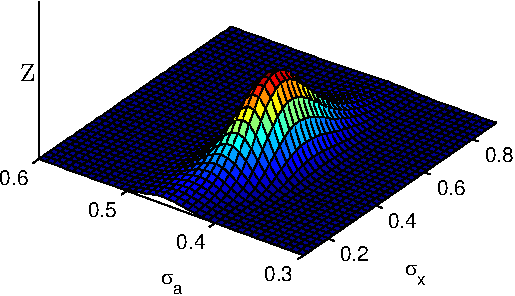
\includegraphics[width=0.33\textwidth]{\infinitefiguresdir/sxsa.pdf} & 
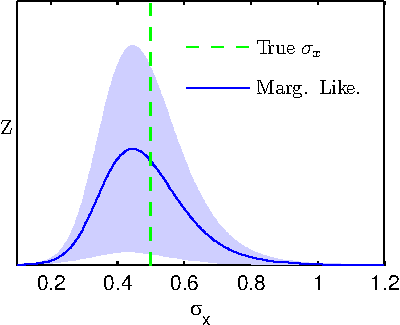
\includegraphics[width=0.3\textwidth]{\infinitefiguresdir/sx.pdf} &
%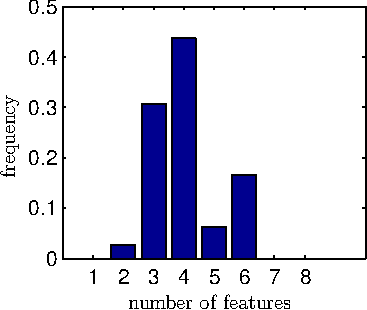
\includegraphics[width=0.4\textwidth]{\infinitefiguresdir/ibp_hist_200.pdf} &
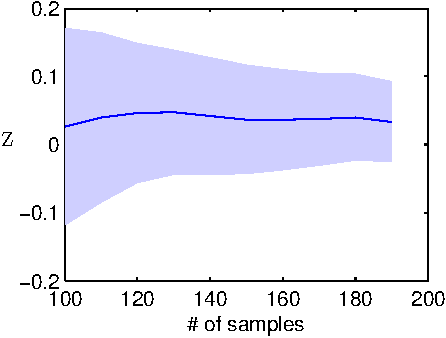
\includegraphics[width=0.3\textwidth]{\infinitefiguresdir/samples_vs_Z.pdf}
\end{tabular}
\caption{Computing marginal likelihoods with BQ.  Left: The marginal likelihood as a function of two nuisance parameters.  Center:  A slice of the 2-D marginal likelihood function, at $\sigma_A = 0.4$.  The true value of $\sigma_X$ lies roughly in the center of the likelihood function.  Right: The marginal likelihood as a function of the number of evaluations of the likelihood function.  The shaded error represents uncertainty about the value of the marginal likelihood. }
\label{fig:ibp_exps}
\end{figure}


\subsection{DP Mixture Experiments}

Figure \ref{fig:ibp_exps} demonstrates the use of \bq{} to examine sensitivity to prior parameters.

\begin{figure}
\centering
\begin{tabular}{cc}
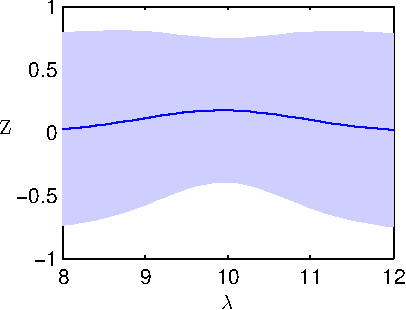
\includegraphics[width=0.33\textwidth]{\infinitefiguresdir/gmm_z_vs_lambda.pdf} & 
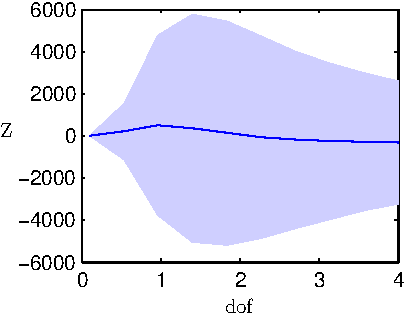
\includegraphics[width=0.33\textwidth]{\infinitefiguresdir/gmm_z_vs_dof.pdf}
\end{tabular}
\caption{A demonstration of computing marginal likelihoods.  Left: The marginal likelihood versus the prior mean.  Right:  Marginal likelihood versus the degrees of freedom of the mixture components.  dof = 1 is Cauchy, dof = 2 is Student's t, dof = $\infty$ is Gaussian.  The shaded error represents uncertainty about the value of the marginal likelihood. }
\label{fig:gmm_exps}
\end{figure}

Figures \ref{fig:ibp_exps} and \ref{fig:gmm_exps} show not only the marginal likelihood of different parameter settings, but also the marginal variance of the likelihood functions.  We must distinguish between two types of uncertainty represented here.  First, the shape of the likelihood function indicates our posterior uncertainty over its parameter, given the data.  Second, the \gp{} posterior uncertainty in the likelihood function(represented by the shaded areas) represents our uncertainty about this likelihood function.  Our uncertainty about the likelihood function can be made arbitrarily small by continuing to sample the likelihood function.  However, we may still remain uncertain about the value of the latent parameter.


Code to produce all experiments will be made available at the authors' website.



%For small numbers of nuisance parameters, we can integrate numerically over them by re-computing likelihoods at the sample locations, with the likelihoods recalculated as a function of the nuisance parameters.  This operation does not require re-computing the Gram matrix or its inverse, so is only as slow as computing the likelihood function.  It also induces a non-\gp{} posterior on the likelihood function.
 
%\subsection{Levels of uncertainty}

\section{Discussion}

Nuisance parameters such as $\sigma_X$ could also be dealt with in the \bq{} by adding them to the kernel and the domain of integration if desired.


\subsection{Appropriateness of the GP prior}

Placing a \gp{} prior on the likelihood function allows us to take advantage of our knowledge of the smoothness of this function.  However, there is ample reason to be believe that the \gp{} prior is inappropriate for modeling likelihood functions. In \cite{BZMonteCarlo} it is suggested to place the \gp{} on the log-likelihood function, which would presumably make the additive form of the kernels given in the paper much more appropriate. This was done by [cite BQR paper], and resulted in better performance, at the cost of a much more complicated inference procedure.

As is generally true for Bayesian methods, there exist many cases where \bq{} will underestimate its uncertainty.  %We have two responses to this problem:  First, we may expect that more sophisticated sampling schemes, and better models of likelihood functions will provide better-calibrated uncertainty estimates in general.
Our response to this objection is that any uncertainty estimate is better than none at all. In our experiments, we observed cases in which the model's posterior uncertainty is significant, alerting us to the fact that we have not yet observed enough about the likelihood function to be certain about its shape.  In the case of MCMC, this sort of uncertainty estimate is typically unavailable.  That is to say, our model cannot account for `unknown unknowns', but it can at least account for `known unknowns', which is a step up from the point estimates provided by MCMC.


\section{Conclusions}
We have extended Bayesian quadrature to infinite, structured domains, and demonstrated that this method can be used for inference in nonparametric models.  We have given necessary conditions for convergence and examples of how to construct kernels which take advantage of the many symmetries of typical likelihood functions.  We demonstrated some properties of this method, which include uncertainty estimates, flexibility in sampling methods, and the ability to re-use samples from on setting to perform post-hoc sensitivity analysis of nuisance parameters.

%\subsection{Future Work}

%The kernels and modes presented here are simply meant as a proof of concept.  Both the \ibp{} kernel and \dirpro{} kernel could benefit from a richer parameterization.  

%We expect that non-parametric \bq{} will find use in any setting where evaluating the likelihood function is expensive.  One promising application would be in reinforcement learning, where one could place a kernel between policies, or between agent trajectories when attempting to estimate expected reward.  Another application may be defining kernels between programs or functions when attempting sequence induction.

%Practical use of \bq{} still faces many issues regarding sampling, model choice, sparsifying approximations and hyperparameter integration.  The situation may be analogous to the usefulness of MCMC around the time when the Metropolis-Hastings sampler was invented.  However, because of its potential to provide an alternative to the \mcmc{} family of inference methods which have been the focus of intense research, we believe that \bq{} is worthy of further development.



\outbpdocument{
\bibliographystyle{plainnat}
\bibliography{references.bib}
}


